\section{Data Collection \& Data Preparation}
\label{sec:data_collection_and_data_preparation}
In this section, we elaborate on different data sources and data cleaning techniques used. We then explain how the trips are calculated from raw data and how they are aggregated to demand and availability datasets.


%% -------------------------------------- bicycle sharing data
\subsection{Data Collection}
We received bicycle rental data from the bicycle sharing provider NextBike for the city of Leipzig during the year 2019.
% 
The bicycle rental data is available as a snapshot of bicycle locations at the start and end of each trip. Additionally, locations at the beginning and end of each day are provided. For two consecutive days, these are only one second apart. However, there is often a difference in distance of multiple kilometers between them, which would be impossible to travel in one second.
% The bicycle rental data is available as a snapshot of bicycle locations at the start and end of a trip as well as the first and last second of a day.
% The last location of a bicycle at a given day is, temporally, only one second apart from the first location of the consecutive day.
% However, that these locations often differ by multiple kilometres, which is impossible to travel in one second.
Therefore, we assume that the first and last entry of a day are not actually one second apart but instead represent relocations that happened at another time. To clean the data, we remove all samples that are not in the time interval from 01.01.2019 to 31.12.2019, as we only analyze the year 2019. Additionally, we compare bicycle locations with the official NextBike flexzone to eliminate samples with erroneous GPS data. The results show, that over \(70\%\) of all samples lie outside of the flexzone. As it is very unlikely that so many samples are erroneous, we decided to add a 10km buffer to the flexzone, so that only samples that are really far away are removed.

%% -------------------------------------- weather data
We have also collected hourly weather data, such as temperature, precipitation,
cloud coverage and wind speed. Our selection is based on the approach taken by
\shortciteA{schroer2022data}, who used these features in their research on
repositioning in on-demand vehicle sharing systems. For this purpose we used
the open portal of the German Weather Service
\shortcite{german_weather_service}.  We used time interpolation to fill missing
values.
% Additionally information about the hourly weather was added to the trip data. For this we included the meteorological features temperature, precipitation, cloud cover and wind speed. This selection is based on the approach taken by \shortciteA{schroer2022data} who used these features for bike sharing predictive analytics. Source of the data is the open data portal of the German Weather service\footnote{\url{https://opendata.dwd.de}}. The weather data then got merged to the trips utilizing the timestamp.

%% -------------------------------------- landuse data
Additionally, we gathered the land use data from the Kopernikus website \shortcite{copernicus_land_use}. It describes for which purpose a certain area is used, such as "construction sites" or "green urban areas".
% We further added land use data to both the trips and the hexagons in all resolutions.
% For this, we downloaded the land use data set for Leipzig from the Kopernikus website \shortcite{copernicus_land_use}.
% For individual trips, we merged this on the start and end location. For hexagons, we calculated for each hexagon which percentage of the area represents which land use type.

%% -------------------------------------- POI data
Lastly, we extracted locations of various points of interest (POI) from an open-source tool called  OpenStreetMap \shortcite{osm}. We decided to focus on five POI categories to preserve the clarity of our findings and to avoid the curse of dimensionality. The categories included are - sustenance, public transport, education, arts and culture, sports.

%% -------------------------------------- trips calculation
\subsection{Trips Calculation}
To generate trips from bicycle locations we designed the following procedure:
% \begin{enumerate}
%     \item Sort all samples by time
%     \item Group all samples by bicycle id
%     \item Create tuples with each two consecutive locations of each bicycle
%     \item Classify tuples as trips or relocations
% \end{enumerate}

\begin{table}[h!]
    \centering
    \begin{tabular}{ |l l| }
        \hline
        1 & Sort all samples by time                                          \\
        \hline
        2 & Group all samples by bicycle ids                                  \\
        \hline
        3 & Create tuples with each two consecutive locations of each bicycle \\
        \hline
        4 & Classify tuples as trips or relocations                           \\
        \hline
    \end{tabular}
\end{table}

\begin{figure}[htp]
    \centering
    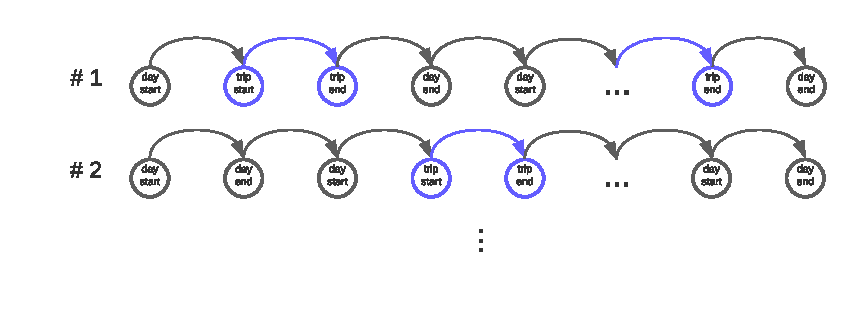
\includegraphics{figures/trip_creation_diagram.pdf}
    \caption{Trips Calculation (trips marked in blue)}
    \label{fig:trip_creation}
\end{figure}

Our rationale is that every pair of consecutive locations of one bicycle has to be either a trip, a relocation or no movement at all.
As we have the information, whether a given sample is the start of a trip, the end of a trip, the start of a day or the end of the day measurement as illustrated in figure \ref{fig:trip_creation}, we can easily classify each pair of consecutive locations.

We then remove all trips that exceed the speed of 25km/h, which is the limit for e-bikes in Germany \shortcite{giant_bicycles}. Trips, that exceed such limit, would require a person to cycle faster than the maximum speed of e-bike without any stops. As this does not seem plausible, we consider these trips faulty.
Also, the distance is measured between the start and the end location, which is a lower bound on the actual distance traveled.
Therefore, the real distance is most likely longer and the real speed is most likely higher.

%% -------------------------------------- demand and availability aggregation
\subsection{Demand And Availability Aggregation}
Next, we aggregate the trips spatially and temporally to determine demand. For spatial aggregation we use the hexagonal hierarchical geospatial indexing system called H3 \shortcite{uber_h3_2022}, which partitions the earth into hexagons. %of varying sizes depending on the chosen resolution
In our research, we use the resolutions 7, 8 and 9, where the edge length of one hexagon corresponds to 1.2km, 460m and 175m respectively.
Additionally, we aggregate trips across time intervals of 1, 2, 6 and 24 hours. Table \ref{table:aggregated_trips} shows a sample of the data that results from this aggregation, which states, for example, that 15 trips started during time interval 2 inside the hexagon with id 871f1ab96ffffff and ended in the hexagon with id 871f1a164ffffff.

\begin{table}[h!]
    \centering
    \begin{tabular}{ |c|c|c|c|c| }
        \hline
        \textbf{start hexagon id} & \textbf{end hexagon id} & \textbf{h3 resolution} & \textbf{time interval} & \textbf{demand} \\
        \hline
        871f1ab96ffffff           & 871f1a164ffffff         & 2                      & 7                      & 15              \\
        \hline
    \end{tabular}
    \caption{Sample of aggregated trip data}
    \label{table:aggregated_trips}
\end{table}
% Real h3 ids actually are in the form of Universally Unique Identifier (UUID), but we've replaced them here with numeric ids for the sake of readability.
% Later we will also use an even more aggregated form of this data, which does not have end hexagon ids.



Also, we calculate the availability of bicycles. For this purpose, we first initialize the availability of all hexagons at all time intervals to the number of bicycles which were seen for the very first time exactly then and there.
% For this purpose, we first initialize the availability of a given hexagon at a given time interval to the number of bicycles whose first seen locations are there.
Next, we update the availability of the hexagons with each trip and relocation by subtracting from the availability in the start hexagon and adding to the availability in the end hexagon.
When a bicycle reaches its final location, it is subtracted from the availability.
Following this approach the availability can be expressed more formally as:
\[A(h, t) = A(h, t-1) + \delta_t^+(h) - \delta_t^-(h) + s_t(h) - d_t(h)\]
where \(A(h, t)\) describes the total number of available bicycles in the hexagon \(h\) during time interval \(t\),
\(\delta_t^+(h)\) and \(\delta_t^-(h)\) describe the total number of incoming and outgoing trips and relocations during time interval \(t\) considering hexagon \(h\),
\(s_t(h)\) describes the number of bicycles that "spawn" (first observation) in hexagon \(h\) during time interval \(t\) and
\(d_t(h)\) describes the number of bicycles that "vanish" (last observation) in hexagon \(h\) during time interval \(t\).

Lastly, we aggregate land use and POI data and merge it on start and end hexagons to trips, demand and availability datasets. Weather data is aggregated temporally and also merged on timestamp and corresponding time interval.
